\documentclass[12pt]{article}
\newif\ifanswer%\answertrue% comment out \answertrue to show/hide answers
\usepackage{../../preamble3}% preamble always after \newif\ifanswer
%\pagenumbering{gobble}
\title{MathCounts Competition Practice III, December 2020 \\ Target Round}
\author{Patrick \& James Toche}
\date{Revised:~\today}

\begin{document}
\maketitle
\begin{minipage}{\textwidth}
\begin{abstract}\setlength{\parindent}{0pt}%
Notes on Target Round of MathCounts Competition Practice III, January 2021. 
Questions are from MathCounts Foundation (\url{https://www.mathcounts.org/}). Copyright restrictions may apply. Written for personal use. 
Please report typos and errors over at \url{https://github.com/ptoche/Math/tree/master/mathcounts}. 
\end{abstract}
\end{minipage}

\thispagestyle{empty}
\clearpage

\section*{Target Round}


%%%%%%%%%%%%%%%%%%%%%%%%%%%%%%%%%%%%%%%%%%%%%%%%%%%%%%%%%%%%%%%%%%%%%%%%
\subsection*{1.}
Helga invested $\$1000$ at $5\%$ interest, compounded annually. What is the total amount that Helga will have earned by the end of the fourth year? Express your answer to the nearest dollar. 

\nopagebreak

\$~\fbox{\phantom{ANSWER}}

\begin{answer}
Compounding over $4$ years (the end of the fourth year includes the whole of the fourth year):
\begin{align*}
1000 (1+0.05)^4 - 1000 \approx 215.506
\end{align*}

\begin{empheq}[box={\mathbox[colback=white]}]{equation*}
   \$~ 216
\end{empheq} 
\end{answer}
%%%%%%%%%%%%%%%%%%%%%%%%%%%%%%%%%%%%%%%%%%%%%%%%%%%%%%%%%%%%%%%%%%%%%%%%


%%%%%%%%%%%%%%%%%%%%%%%%%%%%%%%%%%%%%%%%%%%%%%%%%%%%%%%%%%%%%%%%%%%%%%%%
\subsection*{2.}
What is the absolute difference between the sum of the first $10$ positive multiples of $5$ and the sum of the first $10$ positive, even integers?

\nopagebreak

\fbox{\phantom{ANSWER}}

\begin{answer}
\begin{align*}
\sum_{k=1}^{k=10} (5k-2k) 
  = (5-2)\sum_{k=1}^{k=10} k
  = 3 \times \frac{10 \times 11}{2}
  = 165
\end{align*}
\begin{empheq}[box={\mathbox[colback=white]}]{equation*}
    165
\end{empheq} 
\end{answer}
%%%%%%%%%%%%%%%%%%%%%%%%%%%%%%%%%%%%%%%%%%%%%%%%%%%%%%%%%%%%%%%%%%%%%%%%


%%%%%%%%%%%%%%%%%%%%%%%%%%%%%%%%%%%%%%%%%%%%%%%%%%%%%%%%%%%%%%%%%%%%%%%%
\subsection*{3.}
The Moisture Co. produces disinfecting wipes. If $70$ wipes completely fill a rectangular carton measuring $6$ inches by $4$ inches by $2$ inches, and $100$ wipes completely fill a rectangular carton measuring $6$ inches by $4$ inches by $h$ inches, what is the value of $h$? Express your answer as a decimal to the nearest tenth. 

\nopagebreak

\fbox{\phantom{ANSWER}}~inches

\begin{answer}
A stack of $70$ wipes has a height of $2$ inches, therefore
\begin{align*}
h = \frac{100}{70} \times 2 \approx 2.857
\end{align*}
\begin{empheq}[box={\mathbox[colback=white]}]{equation*}
    2.9 ~\text{inches}
\end{empheq} 
\end{answer}
%%%%%%%%%%%%%%%%%%%%%%%%%%%%%%%%%%%%%%%%%%%%%%%%%%%%%%%%%%%%%%%%%%%%%%%%


%%%%%%%%%%%%%%%%%%%%%%%%%%%%%%%%%%%%%%%%%%%%%%%%%%%%%%%%%%%%%%%%%%%%%%%%
\subsection*{4.}
Carpet costs $\$21.95$ per square yard and the padding to put under it costs $\$2.55$ per square yard. Felix plans to install padding and carpet in the region shown in the figure. What is the total cost of the carpet and padding needed to exactly cover the room? 

\begin{center}
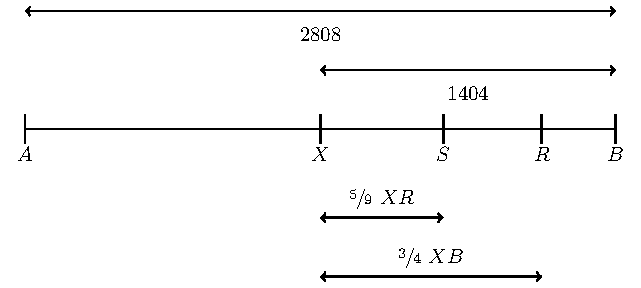
\includegraphics[height=4cm,page=1]{target-04-figure}
\end{center}

\nopagebreak

\$~\fbox{\phantom{ANSWER}}

\begin{answer}
Dividing the area into two rectangles gives a total area, measured in yd$^2$:
\begin{align*}
9 \times 2 + 4 \times 3 = 18 + 12 = 30
\end{align*}
The cost of padding and carpet per square yard is
\begin{align*}
21.95 + 2.55 = 24.5
\end{align*}
The total cost is therefore 
\begin{align*}
24.5 \times 30 = 735
\end{align*}
\begin{empheq}[box={\mathbox[colback=white]}]{equation*}
    \$~735
\end{empheq} 
\end{answer}
%%%%%%%%%%%%%%%%%%%%%%%%%%%%%%%%%%%%%%%%%%%%%%%%%%%%%%%%%%%%%%%%%%%%%%%%


%%%%%%%%%%%%%%%%%%%%%%%%%%%%%%%%%%%%%%%%%%%%%%%%%%%%%%%%%%%%%%%%%%%%%%%%
\subsection*{5.}
In how many different ways can four students stand in a straight line if two of the students refuse to stand next to each other?

\nopagebreak

\fbox{\phantom{ANSWER}}~ways

\begin{answer}
Assign each student to a position in the line, starting with the students who refuse to stand next to each other. If one refusenik student is first or last in the line, there are two places available for the other refusenik, but if the refusenik student is second or third in line, there is only one place available for the other refusenik. After the two refusenik students have been placed in the line, there are two ways to place the other two students. Thus, the total number of ways is:
\begin{align*}
2 \times (2 \times 2 + 2 \times 1) = 12
\end{align*}
\begin{empheq}[box={\mathbox[colback=white]}]{equation*}
    12 ~\text{ways}
\end{empheq} 
\end{answer}
%%%%%%%%%%%%%%%%%%%%%%%%%%%%%%%%%%%%%%%%%%%%%%%%%%%%%%%%%%%%%%%%%%%%%%%%


%%%%%%%%%%%%%%%%%%%%%%%%%%%%%%%%%%%%%%%%%%%%%%%%%%%%%%%%%%%%%%%%%%%%%%%%
\subsection*{6.}
Given that $-3 \leq x \leq 2$ and $20x^2=y-24$, what is the least possible value for $y$? 

\nopagebreak

\fbox{\phantom{ANSWER}}

\begin{answer}
Take $x$ to minimize
\begin{align*}
20x^2 + 24 = y \longrightarrow \min
\end{align*}
or, equivalently, to minimize
\begin{align*}
x^2  \longrightarrow \min
\end{align*}
The minimum occurs for $x=0$, and therefore $y=24$. 
\begin{empheq}[box={\mathbox[colback=white]}]{equation*}
    24 
\end{empheq} 
\end{answer}
%%%%%%%%%%%%%%%%%%%%%%%%%%%%%%%%%%%%%%%%%%%%%%%%%%%%%%%%%%%%%%%%%%%%%%%%


%%%%%%%%%%%%%%%%%%%%%%%%%%%%%%%%%%%%%%%%%%%%%%%%%%%%%%%%%%%%%%%%%%%%%%%%
\subsection*{7.}
Bill, Phill and Jenny are siblings. Bill is twice as old as Phil. Jenny is two years younger than Bill. Currently, their dad is twice as old as the sum of their ages. In nine years, their dad's age will be equal to the sum of his three kids' ages at that time. What is Jenny's current age? 

\nopagebreak

\fbox{\phantom{ANSWER}}~years old

\begin{answer}
Let $b$, $p$, $j$, $d$ denote the current ages of Bill, Phill, Jenny, and their Dad. The verbal statement translates to:
\begin{align*}
b & = 2p \\
j & = b - 2 = 2p - 2\\
d & = 2 (b + p + j) \\
d + 9 & = (b + 9) + (p + 9) + (j + 9)
\end{align*}
Simplifying and substituting yields:
\begin{align*}
b & = 2p \\
j & = b - 2 \Rightarrow 2p = j + 2 \Rightarrow p = (j+2)/2 \\
d & = 2 (b + p + j) \\
d & = (b + p + j) + 18 = d/2 + 18 \\
  \Rightarrow d & = 36 \\
  \Rightarrow (b + p + j) & = 18 = (2p + p + j) = 3p + j \\
  \Rightarrow j & = 18 - 3p = 18 - 3(j+2)/2\\
  \Rightarrow (1+3/2) j & = 15\\
  \Rightarrow         j & = 6\\
\end{align*}
\begin{empheq}[box={\mathbox[colback=white]}]{equation*}
    6 ~\text{years old}
\end{empheq} 
\end{answer}
%%%%%%%%%%%%%%%%%%%%%%%%%%%%%%%%%%%%%%%%%%%%%%%%%%%%%%%%%%%%%%%%%%%%%%%%


%%%%%%%%%%%%%%%%%%%%%%%%%%%%%%%%%%%%%%%%%%%%%%%%%%%%%%%%%%%%%%%%%%%%%%%%
\subsection*{8.}
An ammonia and water mixture fills a five-gallon container. Eighty percent of the mixture is ammonia, but some of the mixture will be drained and replaced with pure water. If a five-gallon mixture of fifty percent ammonia is desired, how many quarts of the mixture need to be drained before the water is added, given that $4$ quarts equals a gallon? Express your answer as a decimal to the nearest tenth. 

\nopagebreak

\fbox{\phantom{ANSWER}}~quarts

\begin{answer}
The quantity of ammonia in the original mixture is $80\%$ of $5$ gallons, or $4$ gallons, or a ratio of $4{:}5$. Since the objective is to obtain a $5$ gallons mixture at $50\%$ contentration, the amount of ammonia needed is $2.5$ gallons. Of the original mixture $4-2.5=1.5$ gallons of ammonia must be drained. Since the ratio of ammonia to water is $4/5$, the ratio of water to ammonia is is $5/4$, so we must remove
\begin{align*}
\frac{5}{4} \times 1.5 = 1.875~\text{gallons}
\end{align*}
Converting gallons to quarts gives
\begin{align*}
 1.875 \times 4 = 7.5
\end{align*}
\begin{empheq}[box={\mathbox[colback=white]}]{equation*}
    7.5 ~\text{quarts}
\end{empheq} 
\end{answer}
%%%%%%%%%%%%%%%%%%%%%%%%%%%%%%%%%%%%%%%%%%%%%%%%%%%%%%%%%%%%%%%%%%%%%%%%

\end{document}